\documentclass[hyperref={unicode}]{beamer}
\usepackage{CJKutf8}
\usepackage{color}
\usepackage{graphicx}
\usepackage{wrapfig}
\usepackage{hyperref}

\usetheme{Madrid}
%\usetheme{Warsaw}
%\usetheme{Singapore}
%\usetheme{Berlin}
\usecolortheme{whale}
% don't need for Madrid, but others need.
% \useoutertheme{infolines} 
% Adding footnotes
\usepackage{textpos} 
%\newenvironment{reference}[2]{% 
 % \begin{textblock*}{\textwidth}(#1,#2) 
  %    \footnotesize\it\bgroup\color{red!50!black}}{\egroup\end{textblock*}} 
% changing the itemization markers
\setbeamertemplate{items}[ball]

% Rounder boxes and shadows
\setbeamertemplate{blocks}[rounded][shadow=true]
% Getting rid of the nabigation icons
\setbeamertemplate{navigation symbols}{}

\begin{document}

\begin{CJK}{UTF8}{gkai}


\title{概率主题模型及其应用}
\author[YiLei,LiXiaodong]{易磊,李晓东}
% \date{\today}
\renewcommand{\today}{ May 24, 2012}
\institute[SSDUT]{大连理工大学软件学院}

\begin{frame}
  \maketitle
\end{frame}

% automatically print the table of contents  at the beginning of each
% section and subsection.
\AtBeginSection[]
{
  \begin{frame}
    \tableofcontents[currentsection,currentsubsection]
  \end{frame}
}

\section{Introduction to topic model}
\subsection{What are topic model?}
\begin{frame}{Information overload}
\begin{columns}
\begin{column}{0.5\textwidth}
  \begin{center}
    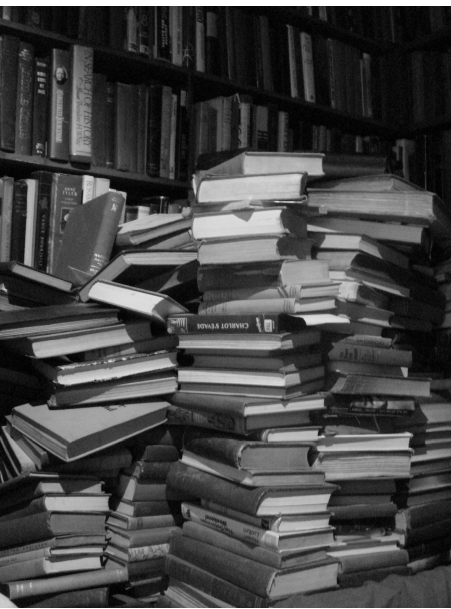
\includegraphics[width=0.8\textwidth]{overload}
  \end{center}
\end{column}
\begin{column}{0.5\textwidth}
  \begin{itemize}
  \item As more information becomes available, it becomes more \alert{difficult} to find and discover what we need.
    \pause
    \item We need new tools to help us \alert{organize}, search, and \alert{understand} these vast amounts of information.
      \pause
      \item Topic modeling provides methods for \alert{automatically organizing}, \alert{understanding}, searching, and summarizing large electronic archives.
  \end{itemize}
\end{column}
\end{columns}
\end{frame}

\subsection{LDA}
\begin{frame}{Latent Dirichilet allocation}
  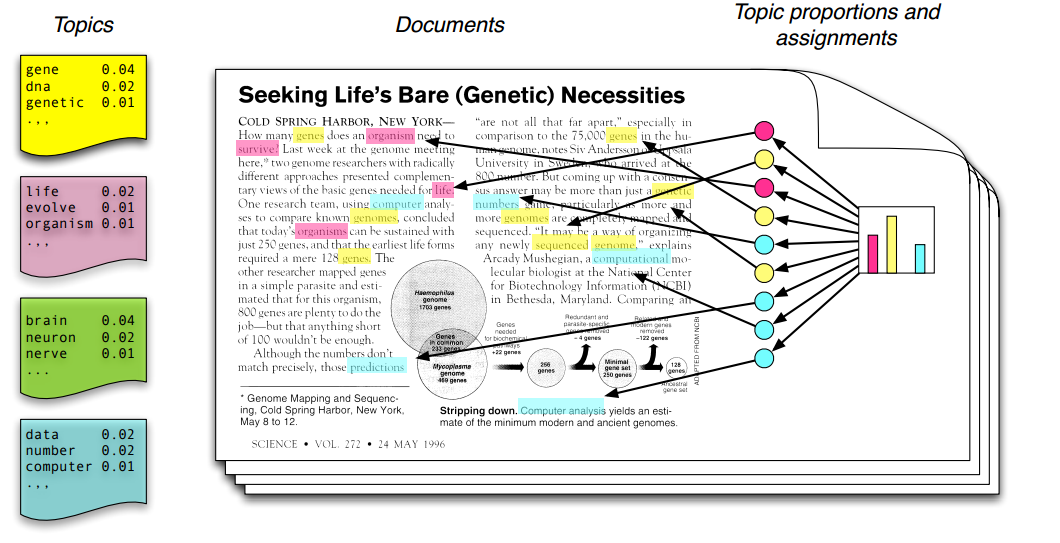
\includegraphics[scale=0.4]{topic_model} 
  \begin{itemize}
  \item Each \alert{topic} is a distribution over words.
  \item Each \alert{document} is a mixture of topics.
  \item Each \alert{word} is drawn from one of those topics.
  \end{itemize}
\end{frame}
\begin{frame}{The posterior distribution}
  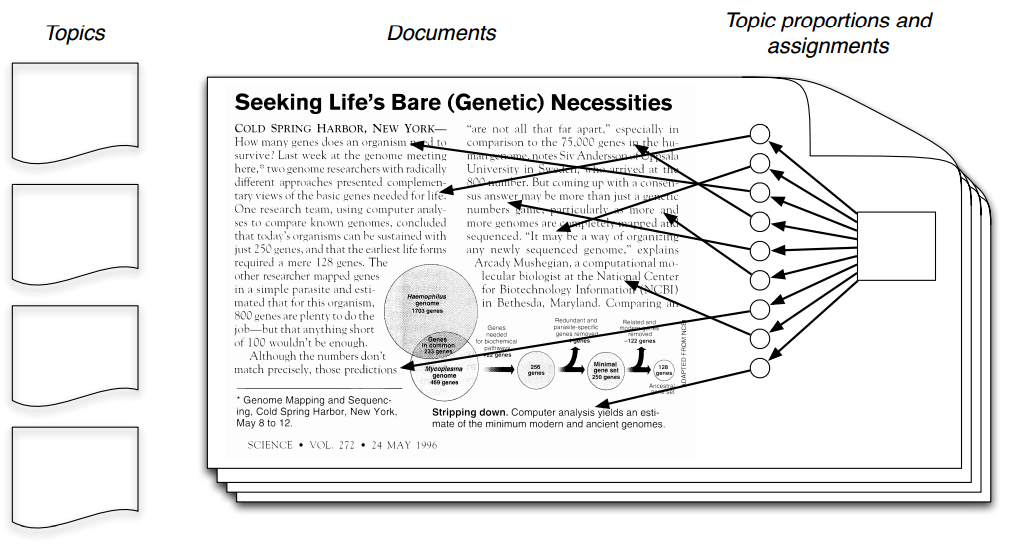
\includegraphics[scale=0.4]{posterior}
  \begin{itemize}
  \item In reality, we \alert{only observe} the documents.
  \item The other structure are \alert{hidden variables}
  \item Our goal is to \alert{infer} the hidden variables.
  \end{itemize}
\end{frame}
\begin{frame}{LDA as a graphicial model}
  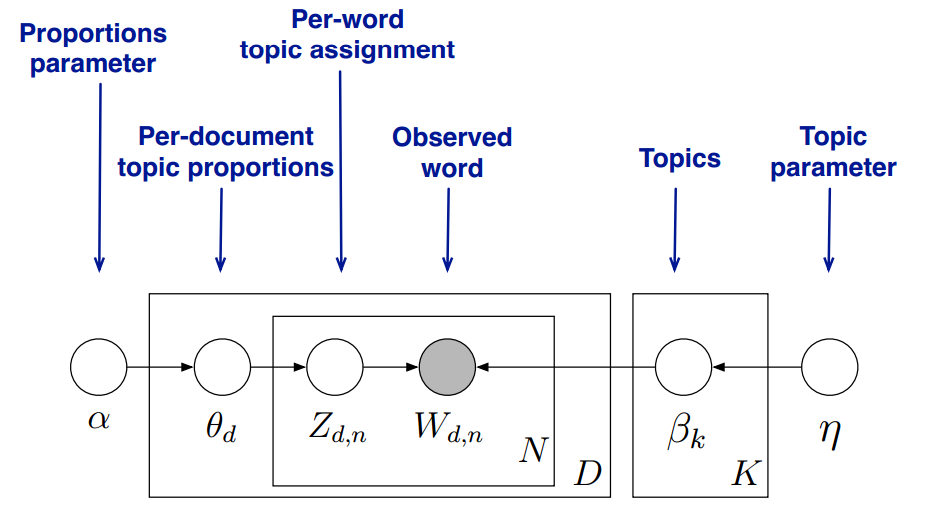
\includegraphics[scale=0.4]{graph}
  \begin{itemize}
  \item Nodes are random variables; \alert{edges} indicate \alert{dependence}.
  \item \alert{Shaded} nodes are observed.
  \item Plates indicate replicated variables.
  \end{itemize}
\end{frame}
\begin{frame}{LDA as a graphicial model}
  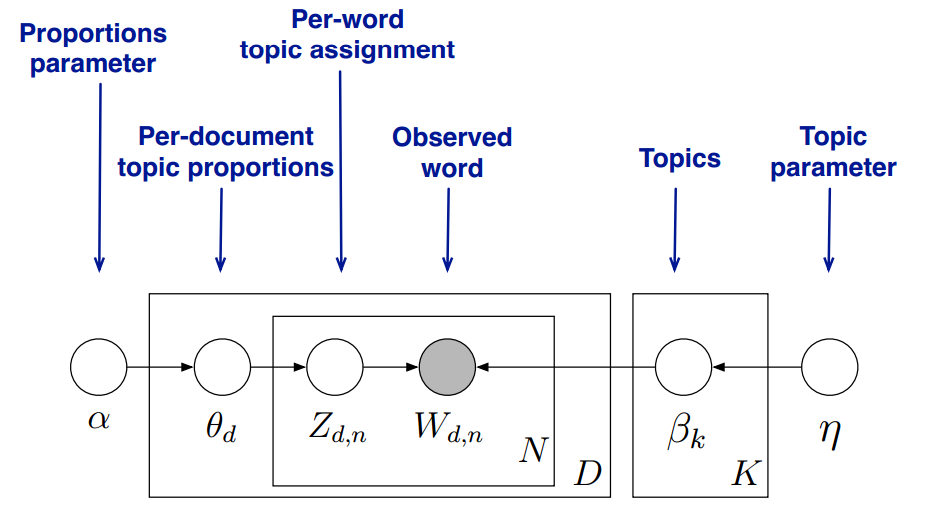
\includegraphics[scale=0.4]{graph}
    \[
    \prod_{i=1}^Kp(\beta_i|\eta)\prod_{d=1}^Dp(\theta_d|\alpha)\Big(\prod_{n=1}^Np(z_{d,n}|\theta_d)p(w_{d,n}|\beta_{1:K},Z_{d,n})\Big)
    \]
\end{frame}

\begin{frame}{LDA}
  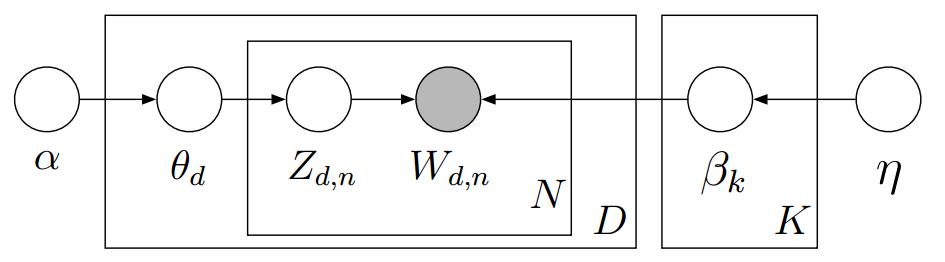
\includegraphics[scale=0.4]{lda}
\begin{block}{This joint defines a posterior.approximate posterior inference algorithms:}
  \begin{itemize}
    \item Gibbs sampling (Griffiths and Stryvers, 2002)
     \item variational inference (Teh et at., 2006)
\end{itemize}
\end{block}
\end{frame}

\section{Applications}
\subsection{Topic model in text mining}
\begin{frame}{分析新浪微博知名微博主的微博主题(just a toy)}
\begin{itemize}
\item 实验数据
  \begin{itemize}
  \item 李开复(创新工场董事长兼首席执行官) 4000条最新微博
  \item 杨幂(中国大陆知名女演员) 2000条最新微博
  \item 36氪(关注互联网创业的科技博客) 7700条最新微博
  \end{itemize}
\item 预处理
\begin{itemize}
\item 分词
\item 去除停用词
\end{itemize}
\item LDA建模,使用LDA的开源实现gensim
\item 实验环境及参数
\begin{itemize}
\item 机器配置: Intel(R) Core(TM)2 Duo CPU E7400 @ 2.80GHz,内存2G,操作系统Ubuntu 11.04
\item 主题个数设为10
\end{itemize}
\end{itemize}
\end{frame}

\begin{frame}{实验结果}
 \begin{itemize}
 \item 李开复的微博主题
   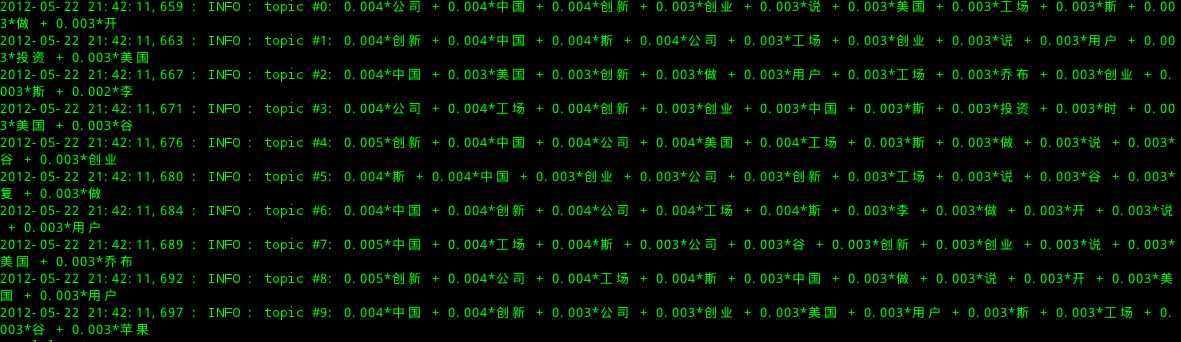
\includegraphics[scale=0.3]{likaifu}
 \item 杨幂的微博主题
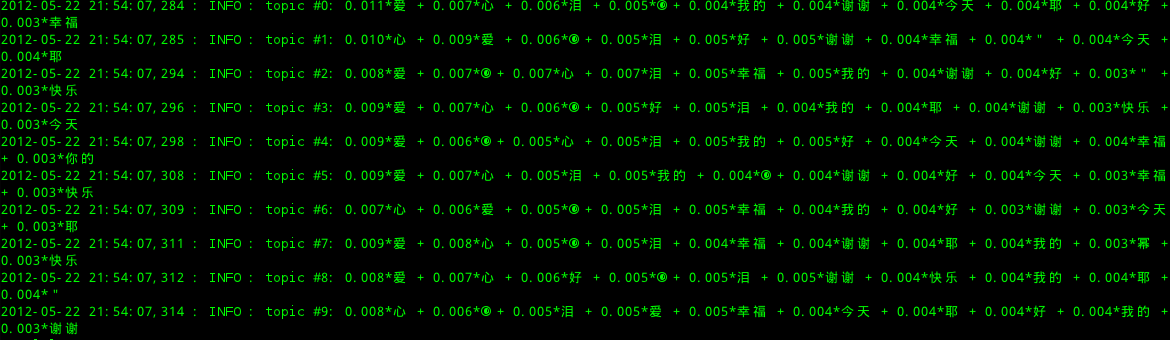
\includegraphics[scale=0.3]{yangmi}
\end{itemize}
\end{frame}
\begin{frame}{实验结果(续)}
 \begin{itemize}
 \item 36氪的微博主题
   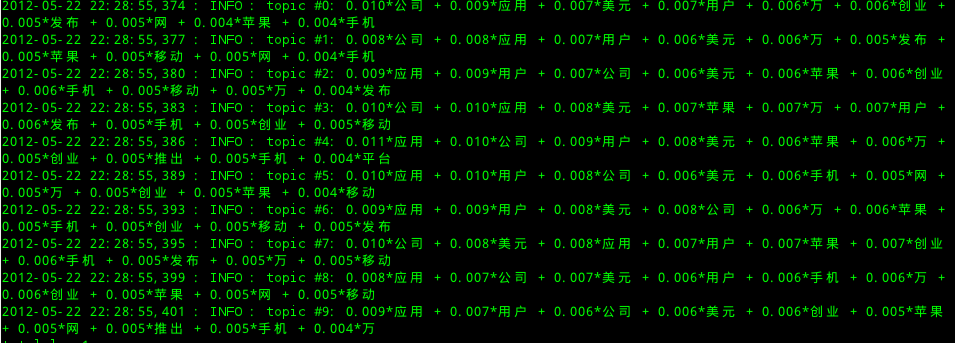
\includegraphics[scale=0.3]{36ke}
\end{itemize}
\end{frame}
\begin{frame}{主题归纳}
\begin{itemize}
\item 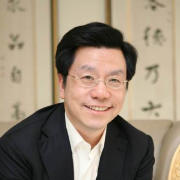
\includegraphics[width=1.0cm]{likaifulogo}
  \alert{创新,中国,创业,投资,用户,硅谷,苹果}
\item 
\includegraphics[width=1.0cm]{yangmilogo}
  \alert{爱,心,幸福,谢谢,快乐,耶}
\item 
\includegraphics[width=1.0cm]{36kelogo}
  \alert{公司,应用,美元,用户,创业,发布,移动,苹果,手机}
\end{itemize}
\end{frame}

\subsection{Topic model in image processing}
\begin{frame}{Topic model in image processing}
  \begin{itemize}
  \item 实验数据: youtube22数据集,包含22个概念的数据,实验只使用其中的一个概念,篮球。一共使用了50个与篮球相关的视频,提取的关键帧包括2632张图片。
  \item 特征提取:我們了提取\alert{SIFT}特征,SIFT算法是一种提取局部特征的算法,在尺度空间寻找极值点,提取位置,尺度,旋转不变量。
  \item 关键帧的向量表示,使用BOF模型。
  \item 实验参数及环境设置:SIFT的采样数目设为1万个,聚类为500类,每张图片用一个500维的特征向量表示。然后通过LDA进行主题分析,主题个数我们设置为10,
\end{itemize}

\end{frame}
\begin{frame}{实验结果}
  \begin{itemize}
  \item Topic 2:   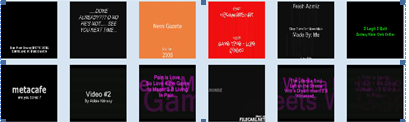
\includegraphics[scale=0.6]{topic2}
  \item Topic 3:   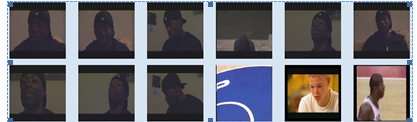
\includegraphics[scale=0.6]{topic3}
  \item Topic 5:   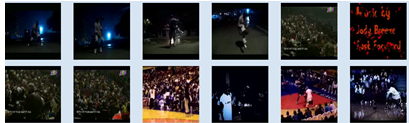
\includegraphics[scale=0.6]{topic5}
  \end{itemize}

\end{frame}
\begin{frame}{实验结果(续)}
  \begin{itemize}
  \item  Topic 1: 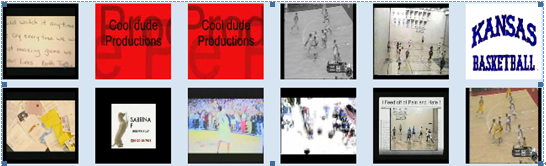
\includegraphics[scale=0.6]{topic1}
  \item Topic 4:   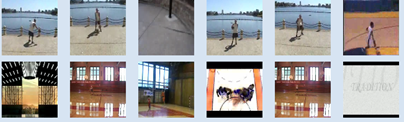
\includegraphics[scale=0.8]{topic4}
  \end{itemize}

\end{frame}
\section{Model extensions}
\begin{frame}{Beyond latent Dirichlet allocation}
  \begin{itemize}
  \item Modeling richer assumptions
    \begin{itemize}
      \item Dynamic topic models
      \item Correlated topic models
    \end{itemize}
  \item Supervised topic models
\begin{itemize}
\item Supervised LDA
\item Relational topic models
\end{itemize}

  \item Bayesian nonparametric topic models
  \end{itemize}

\end{frame}

\section{Conclusion}
\begin{frame}{Summary}
  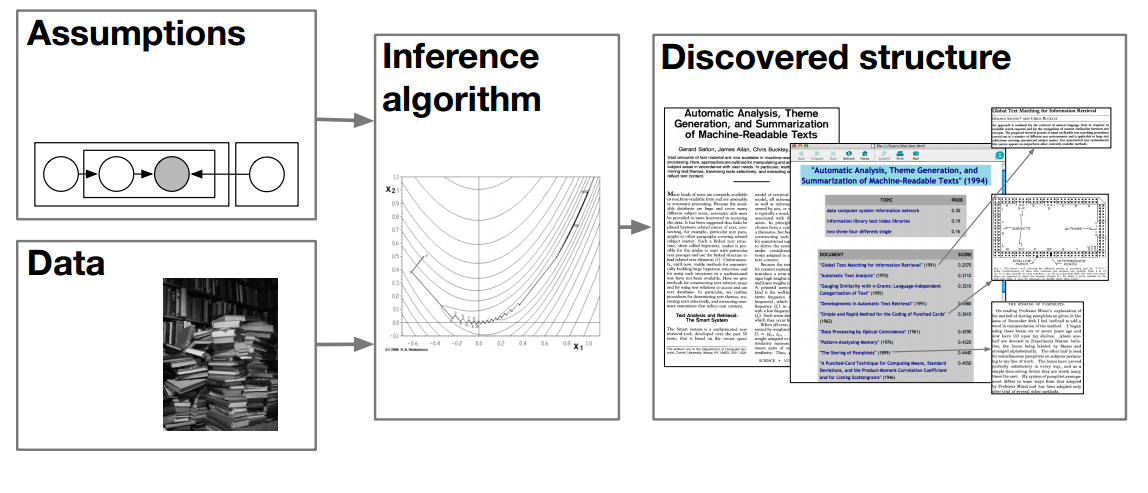
\includegraphics[scale=0.4]{summary}
\end{frame}

\section{Reference}
\begin{frame}{Reference}
\begin{itemize}
\item David M. Blei, Andrew Ng, Michael Jordan. Latent Dirichlet allocation. JMLR (3) 2003 pp. 993-1022.
\item   David M. Blei. Introduction to Probabilistic Topic Models. Communications of the ACM.2011
\item David M. Blei, Jon D. McAuliffe. Supervised Topic Models. NIPS (2007)
\item David M. Blei, John D. Lafferty. Dynamic Topic Models. ICML (2006)
\item Jonathan Chang, David Blei. Relational Topic Models for Document Networks. AIStats (2009)
\end{itemize}
\end{frame}

\section{The end}
\begin{frame}{Q\&A}
  \begin{center}
    \LARGE{\alert{Thanks!}}
  \end{center}
\end{frame}
\end{CJK}
\end{document}

